\documentclass[9pt]{IEEEtran}

\usepackage[english]{babel}
\usepackage{subcaption}
\usepackage{graphicx}
\usepackage{epstopdf}
\usepackage{fancyhdr}
\usepackage{amsmath}
\usepackage{amsthm}
\usepackage{amssymb}
\usepackage{url}
\usepackage{array}
\usepackage{textcomp}
\usepackage{listings}
\usepackage{hyperref}
\usepackage{xcolor}
\usepackage{colortbl}
\usepackage{float}
\usepackage{gensymb}
\usepackage{longtable}
\usepackage{supertabular}
\usepackage{multicol}

\usepackage[utf8x]{inputenc}

\usepackage[T1]{fontenc}
\usepackage{lmodern}
\input{glyphtounicode}
\pdfgentounicode=1

\graphicspath{{./figures/}}
\DeclareGraphicsExtensions{.pdf,.png,.jpg,.eps}

% correct bad hyphenation here
\hyphenation{op-tical net-works semi-conduc-tor trig-gs}

% ============================================================================================

\title{\vspace{0ex}
Exercise 1: Optical Flow}

\author{Katarina Brešar\vspace{-4.0ex}}

% ============================================================================================

\begin{document}

\maketitle

\section{Introduction}

In this assignment we compare two methods for estimating optical flow: Lucas-Kanade and Horn-Shunck. We test them
on different types of images and analyze their performance. 

\section{Experiments}

\subsection{Rotated random noise}
First, we tested the methods on an image of random noise that has been rotated by 1 degree. The results
are visible in~\ref{fig:noise}. We can see that they both produced smooth flow fields showing the rotation of the random image. 

\begin{figure}[h]
    \centering
    \begin{subfigure}[b]{0.2\textwidth}
        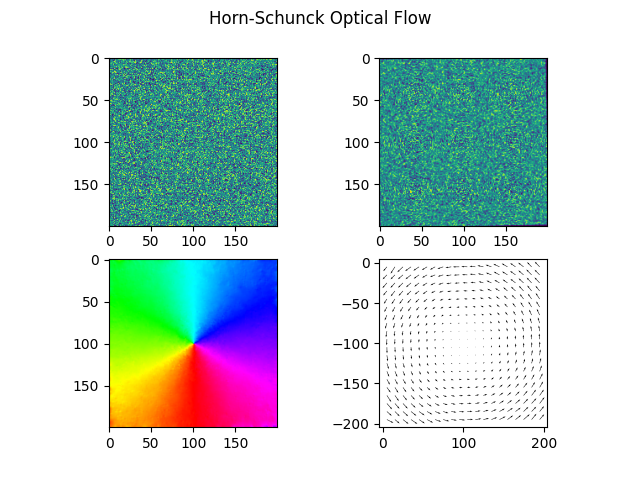
\includegraphics[width=\textwidth]{HS_randomNoise.png}
        \caption{Horn-Shunck method.}\label{fig:noise_hs}
    \end{subfigure}
    \hfill
    \begin{subfigure}[b]{0.2\textwidth}
        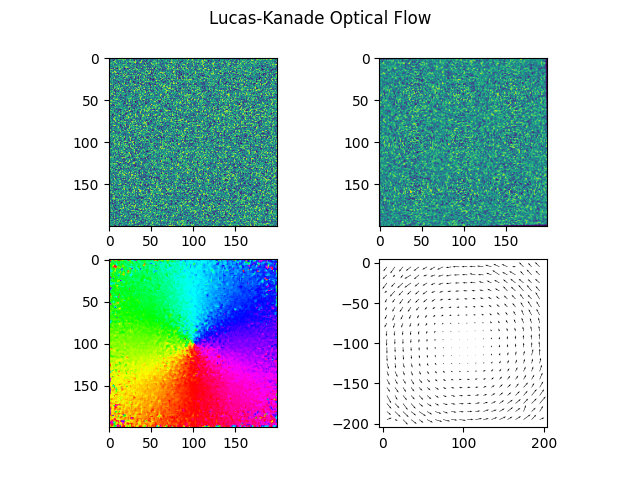
\includegraphics[width=\textwidth]{LK_randomNoise.png}
        \caption{Lucas-Kanade method.}\label{fig:noise_lk}
    \end{subfigure}
    \caption{Optical flow estimation on rotated random noise.}\label{fig:noise}
\end{figure}
    
\subsection{Additional image tests}

\subsection{Reliability of Lucas-Kanade}

In LK flow is computed only where the structure tensor has strong eigen values. To detect this we 
can use the Harris response detector. In figure TODO we can see that the unreliable flow vectors have been removed.
But motion in corners has been preserved? This improves robustness by filtering out flow vectors that are most likely
incorrect. 

\subsection{Parameters analysis}

The LK method has a window size parameter which controls the trade-off between noise and detail. Larger windows may
over smooth and lose fine details, while smaller windows can be more sensitive to noise. There is also the gaussian smoothing sigma
parameter which controls how much the image is smoothed before computing the flow. A larger sigma can help reduce noise but can also blur important features. 
Lastly there is the harris threshold which if too high can discard good flow, while if too low can keep unreliable flow vectors.
TODO show how the flow changes with different parameters.

The HS method has the smoothness regularization parameter $\lambda$. It's a weighing factor which decides how much importance
do we give to the brightness constancy constrain and how much to the smoothness constraint. A larger $\lambda$ will produce
smoother flow fields, but can also lose details. On the other hand a smaller $\lambda$ can capture more details but 
is more sensitive to noise. The HS method also has the number of iterations parameter which controls how many times
the flow is updated. More iterations leads to better convergence but also increases computational cost. 
TODO show how the flow changes with different $\lambda$.


\subsection{Runtime and initialization}
The LK method is generally faster than HS since it computes flow only at certain points and uses a local window. The HS
method uses iterative optimization which can be computationally expensive, especially for larger images. The runtime for both
can be affected by the choice of parameters, such as window size for LK and number of iterations for HS.
TODO time measurments for both methods in an array like table. Add initialization with LK output for HS and add
another column for that. 

\subsection{Pyramidal Lucas-Kanade}
The standard LK method works well only for small motions. If an object moves fast, the small motion assumption is violated. A pyramidal
implementation addressed this issue by created a pyramid of images at different scales. This can be seen in figure TODO. 
Standard LK fails to capture the motion of the fast moving object, while the pyramidal implementation can capture it. 

TODO
Running LK multiple times at the same scale can help slightly but not drastically enough that it would be useful. It
can refine small errors and improves convergence slightly, but it doesn't resolve the large displacement issue. 






\section{Conclusion}

Lucas-Kanade is fast and captures local motion accurately, but it can struggle with large displacements. Horn-Shunck
is more robust to noise and can capture global motion, but it is computationally expensive. Adding Harris-based filtering
improves LK reliability, while initializing HS with LK output can speed up convergence. Overall combining the strength
of both methods can lead to better optical flow estimation.

\bibliographystyle{IEEEtran}
\bibliography{bibliography}

\end{document}
